\section{Standard di qualità}

\subsection{ISO/IEC 9126}
ISO/IEC 9126 è lo standard generale usato per valutare la qualità del software. Esso è articolato in quattro parti:
\begin{itemize}
	\item{Modello per la qualità del software}
	\item{Metriche per la qualità interna}
	\item{Metriche per la qualità esterna}
	\item{Metriche per la qualità in uso}
\end{itemize}

	\subsubsection{Modello per la qualità del software}
	Il modello di qualità stabilito nella prima parte dello standard ISO/IEC 9126 è composto da sei caratteristiche generali e varie sotto caratteristiche misurabili attraverso delle metriche. Tali caratteristiche sono:
	
	\subsubsubsection*{Funzionalità}
	E' la capacità di un prodotto software di fornire funzioni che soddisfano esigenze stabilite nell'\AdR{} e che permettono di operare in condizioni specifiche. Questa capacità si traduce nelle seguenti caratteristiche:
	\begin{itemize}
		\item{\textbf{Appropriatezza}: capacità di fornire funzioni appropriate per attività specifiche che permettano di raggiungere gli obiettivi prefissati;}
		\item{\textbf{Accuratezza}: capacità di fornire risultati corretti e con la precisione richiesta;}
		\item{\textbf{Interoperabilità}: capacità di interagire con uno o più sistemi specificati;}
		\item{\textbf{Conformità}: capacità di aderire a standard;}
		\item{\textbf{Sicurezza}: capacità di proteggere informazioni e dati.}
	\end{itemize}
	
	\subsubsubsection*{Affidabilità}
	E' la capacità del prodotto software di mantenere uno dato livello di prestazioni quando usato in specifiche condizioni. Questa capacità si traduce nelle seguenti caratteristiche:
	\begin{itemize}
		\item{\textbf{Maturità}: capacità di evitare il verificarsi di errori o malfunzionamenti in fase di esecuzione;}
		\item{\textbf{Tolleranza agli errori}: capacità di mantenere livelli predeterminati di prestazioni anche in presenza di malfunzionamenti o errori;}
		\item{\textbf{Recuperabilità}: capacità di ripristinare il livello di prestazioni e di recupero delle informazioni rilevanti in seguito ad un malfunzionamento;}
		\item{\textbf{Aderenza}: capacità di aderire a standard e regole inerenti all'affidabilità.}
	\end{itemize}
	
	\subsubsubsection*{Efficienza}
	E' la capacità di eseguire i compiti prefissati minimizzando il tempo necessario e sfruttando al meglio le risorse disponibili. Questa capacità si traduce nelle seguenti caratteristiche:
	\begin{itemize}
		\item{\textbf{Nel tempo}:}
		\item{\textbf{Nello spazio}:}
	\end{itemize}
	
	\subsubsubsection*{Usabilità}
	Questa capacità si traduce nelle seguenti caratteristiche:
	\begin{itemize}
		\item{\textbf{Comprensibilità}:}
		\item{\textbf{Apprendibilità}:}
		\item{\textbf{Operabilità}:}
		\item{\textbf{Attrattività}:}
		\item{\textbf{Conformità}:}
	\end{itemize}

	\subsubsubsection*{Manutenibilità}
	Questa capacità si traduce nelle seguenti caratteristiche:
	\begin{itemize}
		\item{\textbf{Analizzabilità}:}
		\item{\textbf{Modificabilità}:}
		\item{\textbf{Stabilità}:}
		\item{\textbf{Testabilità}:}
	\end{itemize}

	\subsubsubsection*{Portabilità}
	Questa capacità si traduce nelle seguenti caratteristiche:
	\begin{itemize}
		\item{\textbf{Adattabilità}:}
		\item{\textbf{Installabilità}:}
		\item{\textbf{Conformità}:}
		\item{\textbf{Sostituibilità}:}
	\end{itemize}
	
	\subsubsection{Metriche per la qualità interna}
	
	\subsubsection{Metriche per la qualità esterna}
	
	\subsubsection{Metrica per la qualità in uso}

	\begin{figure}[H]
		\centering
		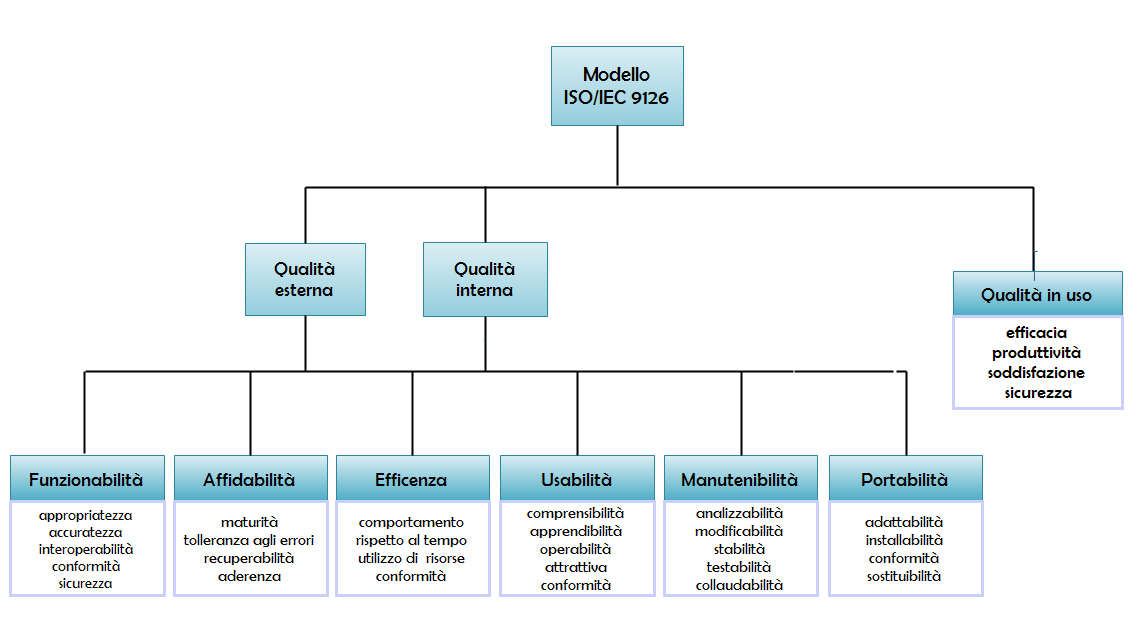
\includegraphics[scale=0.5]{./res/img/ISO_IEC_9126.png}
		\caption[Modello ISO/IEC 9126]{Modello ISO/IEC 9126 (fonte: Wikipedia)}
	\end{figure}

\subsection{ISO/IEC 15504}

\subsection{Ciclo di Deming}